\documentclass{beamer}

\usepackage{amsmath, amssymb}
\usepackage{tikz-cd}
\usepackage{xcolor}
\usepackage{graphicx}

\title{MAT434: Theory of Mathematical Statistics}
\author{\textbf{Miraj Samarakkody}}
\institute{Tougaloo College}
\date{02/12/2025}

\begin{document}

\begin{frame}
    \titlepage
\end{frame}

\begin{frame}{The Binomial Distribution}
    Suppose the \(n\) independent experiments are performed, each resulting in a success with probability \(p\). Let \(X\) be the number of successes in the \(n\) experiments.\\
    \vspace{0.1in}
    \pause
    The probaility that \(p(k)\) can be found in the following way:\\
    \vspace{0.1in}\pause
    Any particular sequence of \(k\) successes and \(n-k\) failures has probability \(p^k(1-p)^{n-k}\) from the multiplication principle. \\
    \pause
    \vspace{0.1in}
    The number of such sequences is \(\binom{n}{k}\).\\\pause
    \vspace{0.1in}
    Thus \[
    P(X=k)=p(k)=\binom{n}{k}p^k(1-p)^{n-k}
    \]

\end{frame}

\begin{frame}{Example}
    Let \(n=10\) and \(p=0.1\). \pause
    \begin{figure}
        \centering
        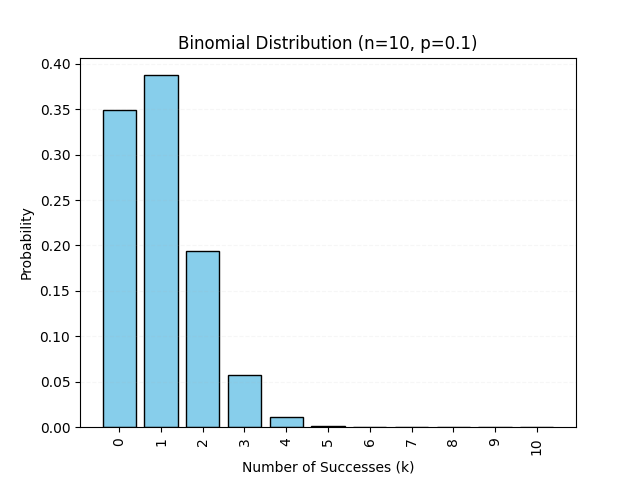
\includegraphics[width=0.5\textwidth]{Figures/Figure_1.png}
        \caption{The Binomial Distribution for \(n=10\) and \(p=0.1\)}
        \label{fig:binomial}
    \end{figure}
\end{frame}

\begin{frame}{Example}
    Let \(n=10\) and \(p=0.5\). \pause
    \begin{figure}
        \centering
        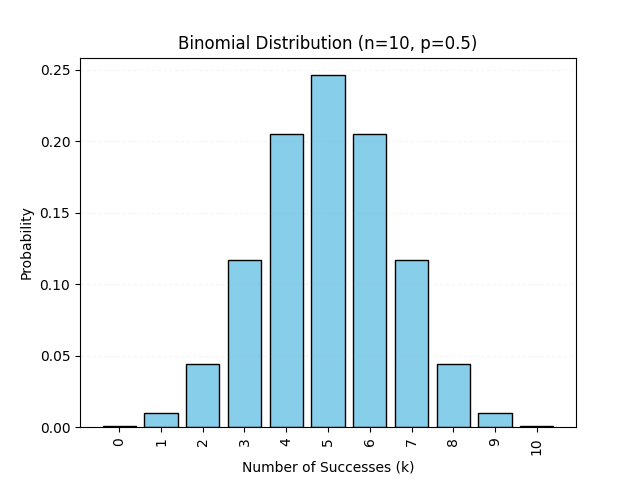
\includegraphics[width=0.5\textwidth]{Figures/Figure_2.png}
        \caption{The Binomial Distribution for \(n=10\) and \(p=0.5\)}
        \label{fig:binomial}
    \end{figure}
\end{frame}

\begin{frame}{Example}
    Let \(n=10\) and \(p=0.8\). \pause
    \begin{figure}
        \centering
        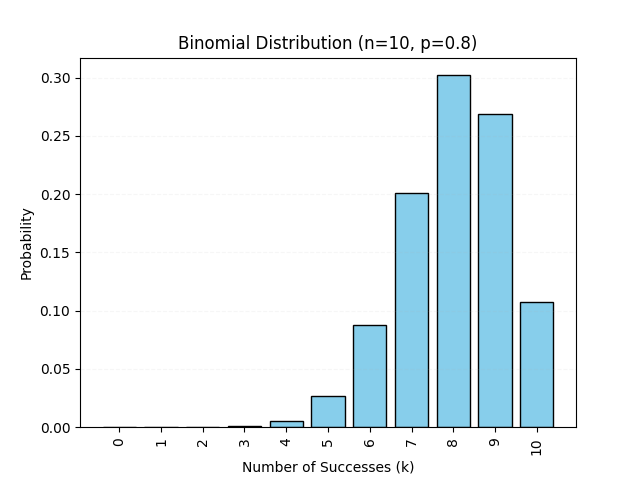
\includegraphics[width=0.5\textwidth]{Figures/Figure_3.png}
        \caption{The Binomial Distribution for \(n=10\) and \(p=0.8\)}
        \label{fig:binomial}
    \end{figure}
\end{frame}


\end{document}